\anonsection{Предлагаемые подходы и методы }

    Для проведения транзакций(исполнения Smart-контрактов) NEAR protocol предоставляет near-cli\footnote{https://github.com/near/near-cli} и near-api-js\footnote{https://github.com/near/near-api-js}~\cite*{docsnear}. Для наших целий требуется near-api-js, а следовательно вытекает потребность использовать язык javascript(nodejs, typescript) для написания <<frontend>> части бота.

    Для реализации самого бота, как следует из названия проекта, используется Discord API. Но конечно, будет использоваться обертка над HTTP запросами. Существует множество всевозможных модулей для разнообразных языков. Для наших целей нам понадобится discord.js(javascript/nodejs)\footnote{https://discord.js.org/}. Также было принято решение, взять обвязку над этой библиотекой - discord.ts(typescript)\footnote{https://discord-ts.js.org/}

	\anonsubsection{Аккаунт}

		Аккаунты в NEAR protocol устроены так, что они имеют человеко-читаемый ID в отличие от большинства других блокчейнов, где обычно используется некоторый hash. Длина логина от 2 до 64 символов и содержит в конце суффикс обозначающий сеть блокчейна: main, test, beta. Аккаунт может создавать подаккаунты, которые по своему функционалу ничем не отличаются от обычного аккаунта. Но они нам понадобятся так как, на один аккаунт можно развернуть только один smart-контракт, а связанно это с тем, что при предложении подписания smart-аккаунта мы будем указывать название аккаунта, что сразу обозначает, который smart-контракт мы хотим инициировать для подписания. И самое главное, что нам нужно так это dev аккаунты. С помощью этих тестовых аккаунтов мы и будем тестировать наши smart-контракты. Они создаются с помощью ранее упомянутого near-cli~\cite*{docsnear}.
		Для того, чтобы мы могли предлагать на подпись smart-контракты, нам нужно, чтобы этот пользователь авторизовался в NEAR wallet или иными словами подписать некоторую транзакцию на образование Access Key.

	\anonsubsection{Access Key}
		Каждый аккаунт имеет создавать множество public/private ключей, которые в Near называются Access Key. Существует два типа Access Key: FullAccess и FunctionCall. Из названия первого можно предположить, что он дает полный доступ и он нам не годится, так как пользователи попросту не будут доверять нашему приложению. FunctionalCall ключ уникален и дает разрешения только на подписание функций контрактов, которые не являются <<payable>>. Он имеет несколько атрибутов: количество Near, которые разрешается тратить на Gas, название контракта, чьи функции разрешается вызывать и названия этих функций, которые будут вызываться. Рисунок \ref{fig:eth_near_cmp}

	\anonsubsection{Хранение в блокчейне}
		Важным вопросом, который не затрагивался при описании стандарта является хранение медиа объекта.В описанном стандарте хранится url на медиа объект, но никак не сам этот медиа объект, связанно это с тем, что хранение объекта невероятно дорогое. Авторы стандарта предлагают несколько подходов, один из них: пользователь изначально просто дает url и мы храним его, но в данном решении есть огромный минус - это то, что мы накладываем обязательство на пользователя об поддержании данного url валидным. Следующий подход заключается в том, что мы - сервис будем хранить данные в централизованном хранилище и тогда нашим опознавательным знаком будет какой-нибудь ключ, который будет соответствовать адресу NFT. И в этом подходе есть тоже минус в виде того, что непонятно какого размера должно быть это хранилище, какие ограничения вводить на размер медиа файла. И последнее предложение, так это хранить в специальном децентрализованном контенто-адресованном хранилище. Одним из примеров таких хранилищ является filecoin\footnote{\url{https://filecoin.io/}}. Минусом данного решения, наверное, является то, что мы начинаем использовать еще один блокчейн, который требует времени для понимания его спецификации. Наша команда приняла решение двигаться от самого простого подхода, то есть использование отданного пользователем url, к более сложному - использование filecoin.

	\anonsubsection{Машинное обучение в маркетплейсе}
		За данную часть я отвечаю в меньшей степени. Но в рамках данного проекта нашей командой принято решение реализовать две идеи: рекомендательную систему или GAN. Рекомендательная система также делится на две части - это предсказание цены за конкретную NFT и более сложная идея - это рекомендовать сам NFT-токен. Идея с GAN выглядит гораздо легче, сравнивая с рекомендательной системой, например, создание аниме персонажа, пиксель арта, которое в последствии пользователь сможет использовать в своих коллекциях или для продажи.

	\begin{figure}[h!]
		\centering
		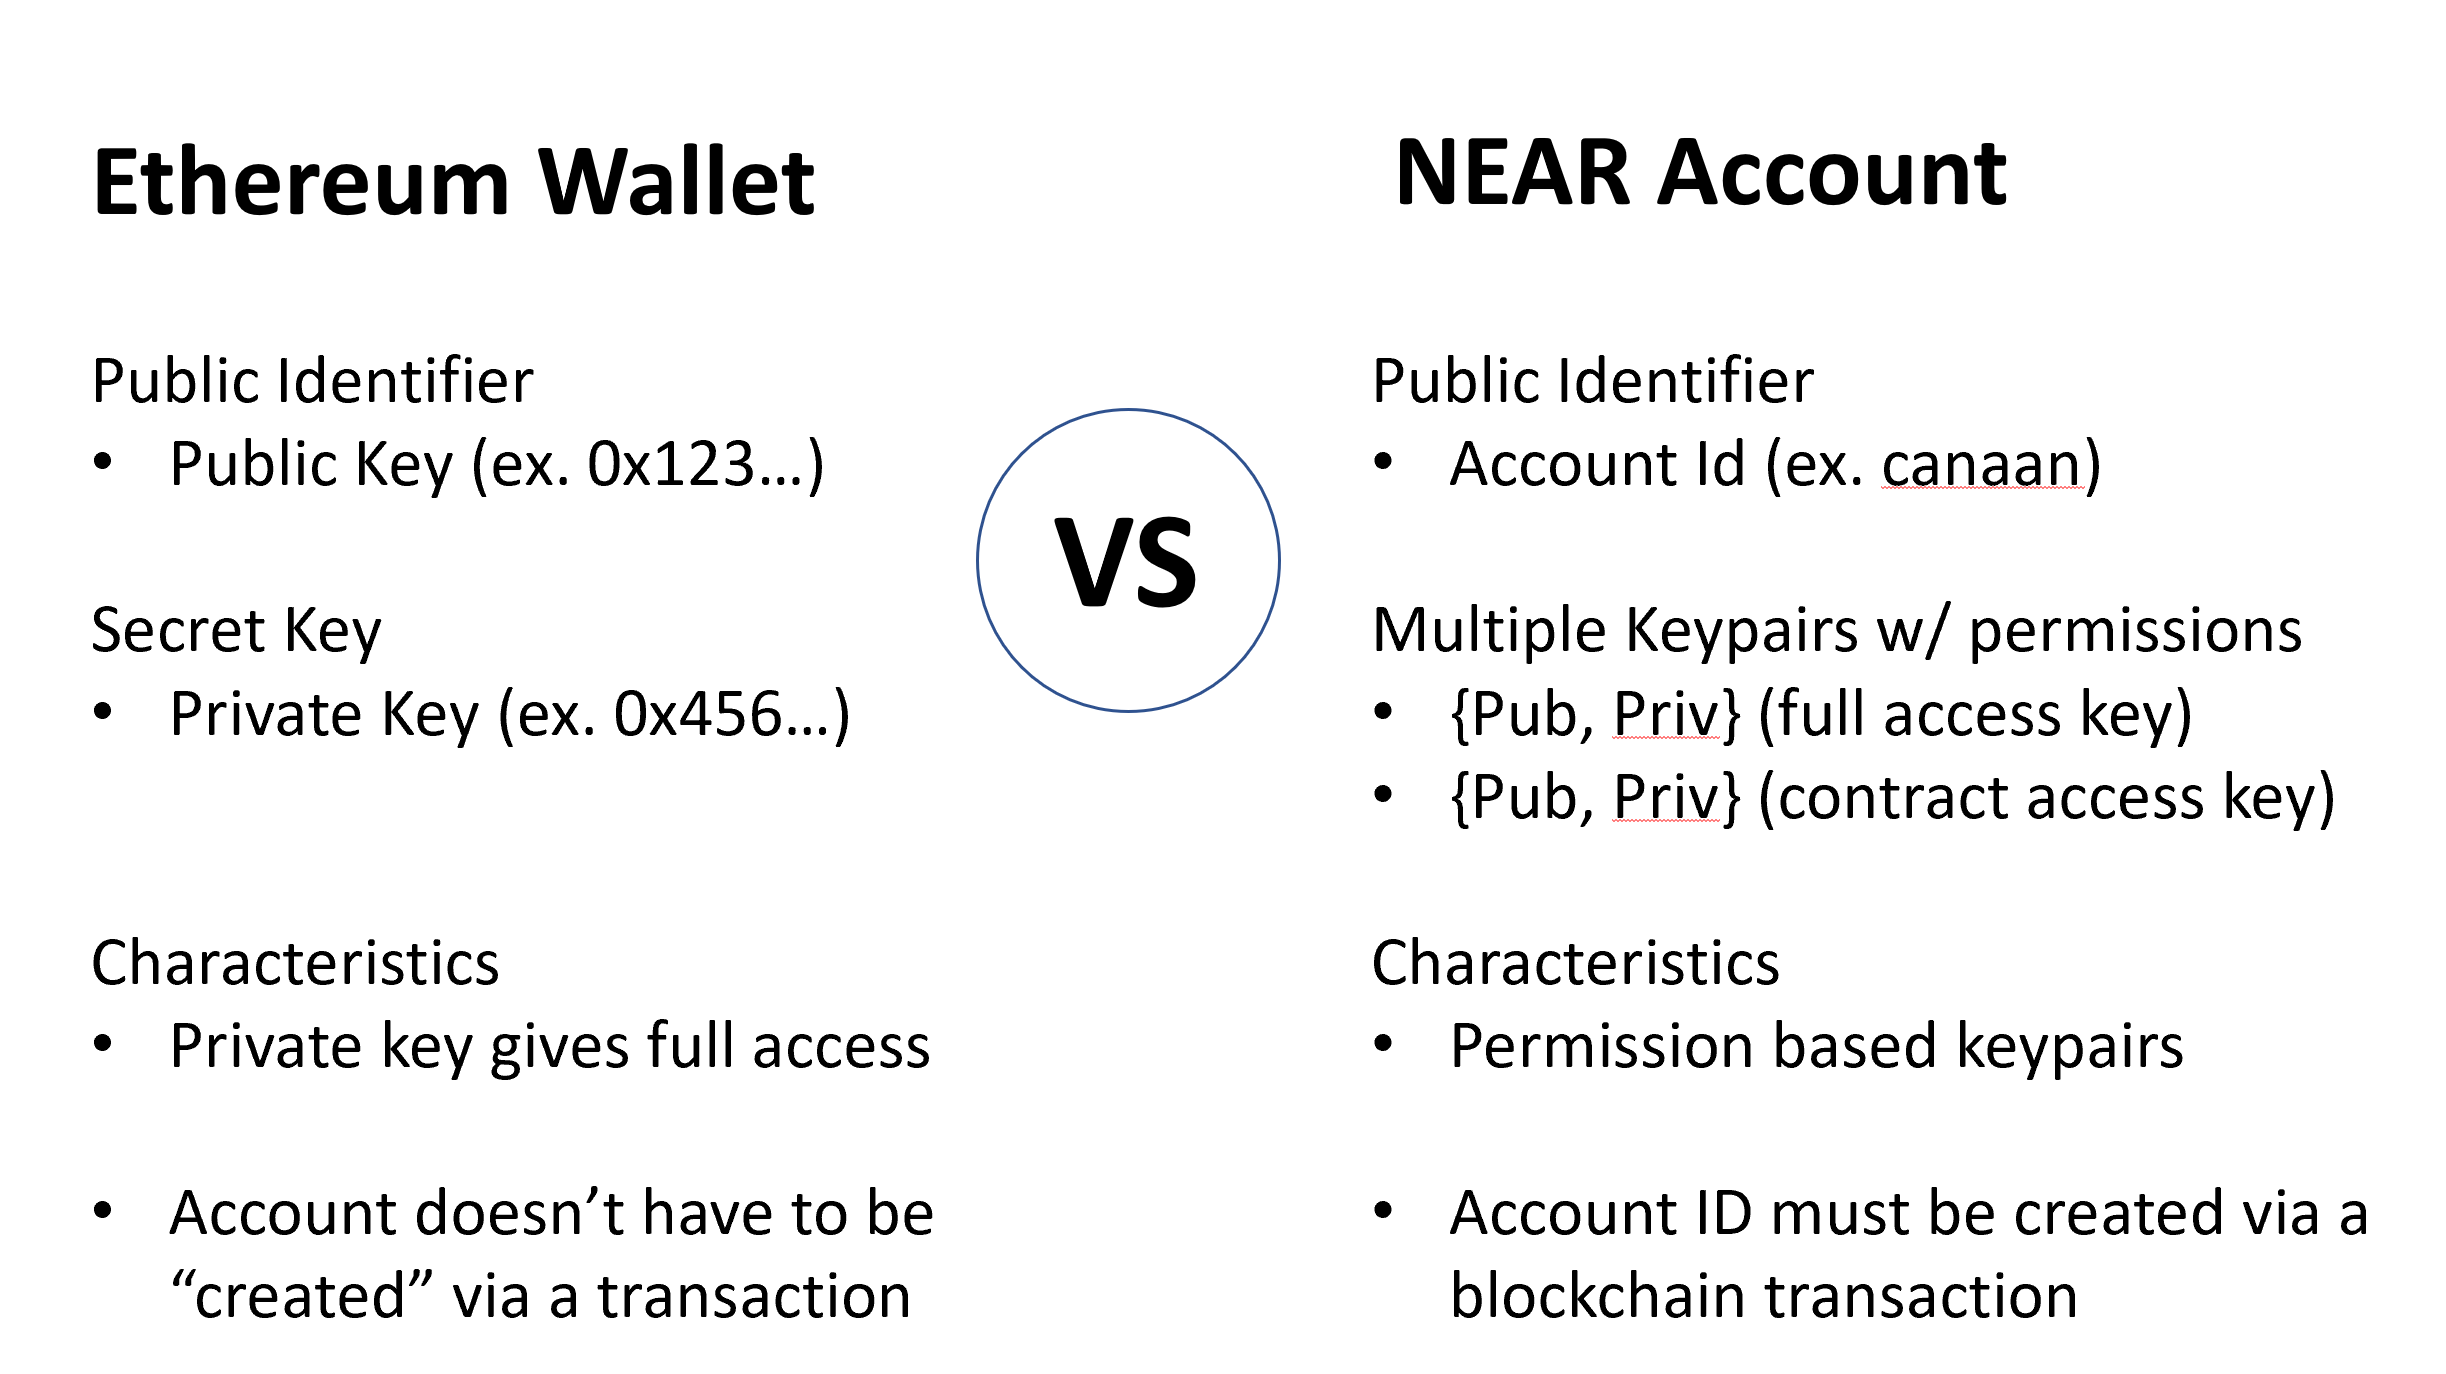
\includegraphics[scale=0.15]{fig/eth_near_cmp.png}
	\caption{Сравнение спецификации аккаунтов и public/private ключей в блокчейнах Ethereum и Near. Источник: \url{medium.com/@clinder}}
		\label{fig:eth_near_cmp}
	\end{figure}
